\section{Implementation of virtual reality application}

\subsection{Technologies}
\subsubsection{Three.js}
Three.js is cross-browser JavaScript library/API used to create and display animated 3D computer graphics in a web browser. It uses WebGL.

\subsubsection{A-Frame}
A-Frame is a web framework for building virtual reality experiences. It was started by Mozilla to make WebVR content creation easier, faster, and more accessible. A-Frame lets you build scenes with just HTML while having unlimited access to JavaScript, Three.js, and all existing Web APIs. It uses an entity-component-system pattern that promotes composition and extensibility. It is free and open source with a welcoming community and a thriving ecosystem of tools and components.

\subsubsection{React}
ReactJS is a javascript library for building user interfaces, originally created by engineers at Facebook to solve the challenges involved when developing complex user interfaces with datasets that change over time. It provides a way to write encapsulated components that manage their own state, then compose them to make complex user interfaces. It doesn't make assumptions about the rest of the technology stack, because it’s just library. Since component logic is written in JavaScript instead of templates, we can easily pass rich data through our app and keep state out of the DOM.

\subsubsection{Redux}
Redux is a predictable state container for JavaScript apps. It helps us write applications that behave consistently, run in different environments (client, server, and native), and are easy to test. On top of that, it provides a great developer experience, such as live code editing combined with a time traveling debugger. We are using Redux together with React, but in general it can be used with any other view library.

The whole state of application is stored in an object tree inside a single store. The only way to change the state tree is to emit an action, an object describing what happened. To specify how the actions transform the state tree, we write pure reducers.

Instead of mutating the state directly, we specify the mutations we want to happen with plain objects called actions. Then we write a special function called a reducer to decide how every action transforms the entire application's state.

The beauty and strength of this pattern is how well it scales to large and complex apps. It also enables very powerful developer tools, because it is possible to trace every mutation to the action that caused it. We can record user sessions and reproduce them just by replaying every action.

\subsubsection{Webpack}
Webpack is a module bundler for modern JavaScript applications. It takes modules with dependencies and generates static assets representing those modules [\ref{r:1}]. Its strength is that it's configurable and developers using it in their applications should know the four core concepts used when configuring Webpack:

\begin{itemize}
\item Entry - Webpack creates a graph of all of your application's dependencies and the starting point of this graph is called entry point. It tells Webpack where to start and follows the graph of dependencies to know what to bundle.
\item Output - it tells Webpack where to bundle our application.
\item Loaders - Webpack treats every file (.css, .html, .scss, .jpg, etc.) as a module. However, webpack only understands JavaScript, so loaders transform these files into modules as they are added to dependency graph.
\item Plugins - loaders only execute transform on per-file basis, but plugins are mostly used to perform actions and custom functionality on combilations or chunks of bundled modules.
\end{itemize}

\begin{figure}[ht!]
\centering
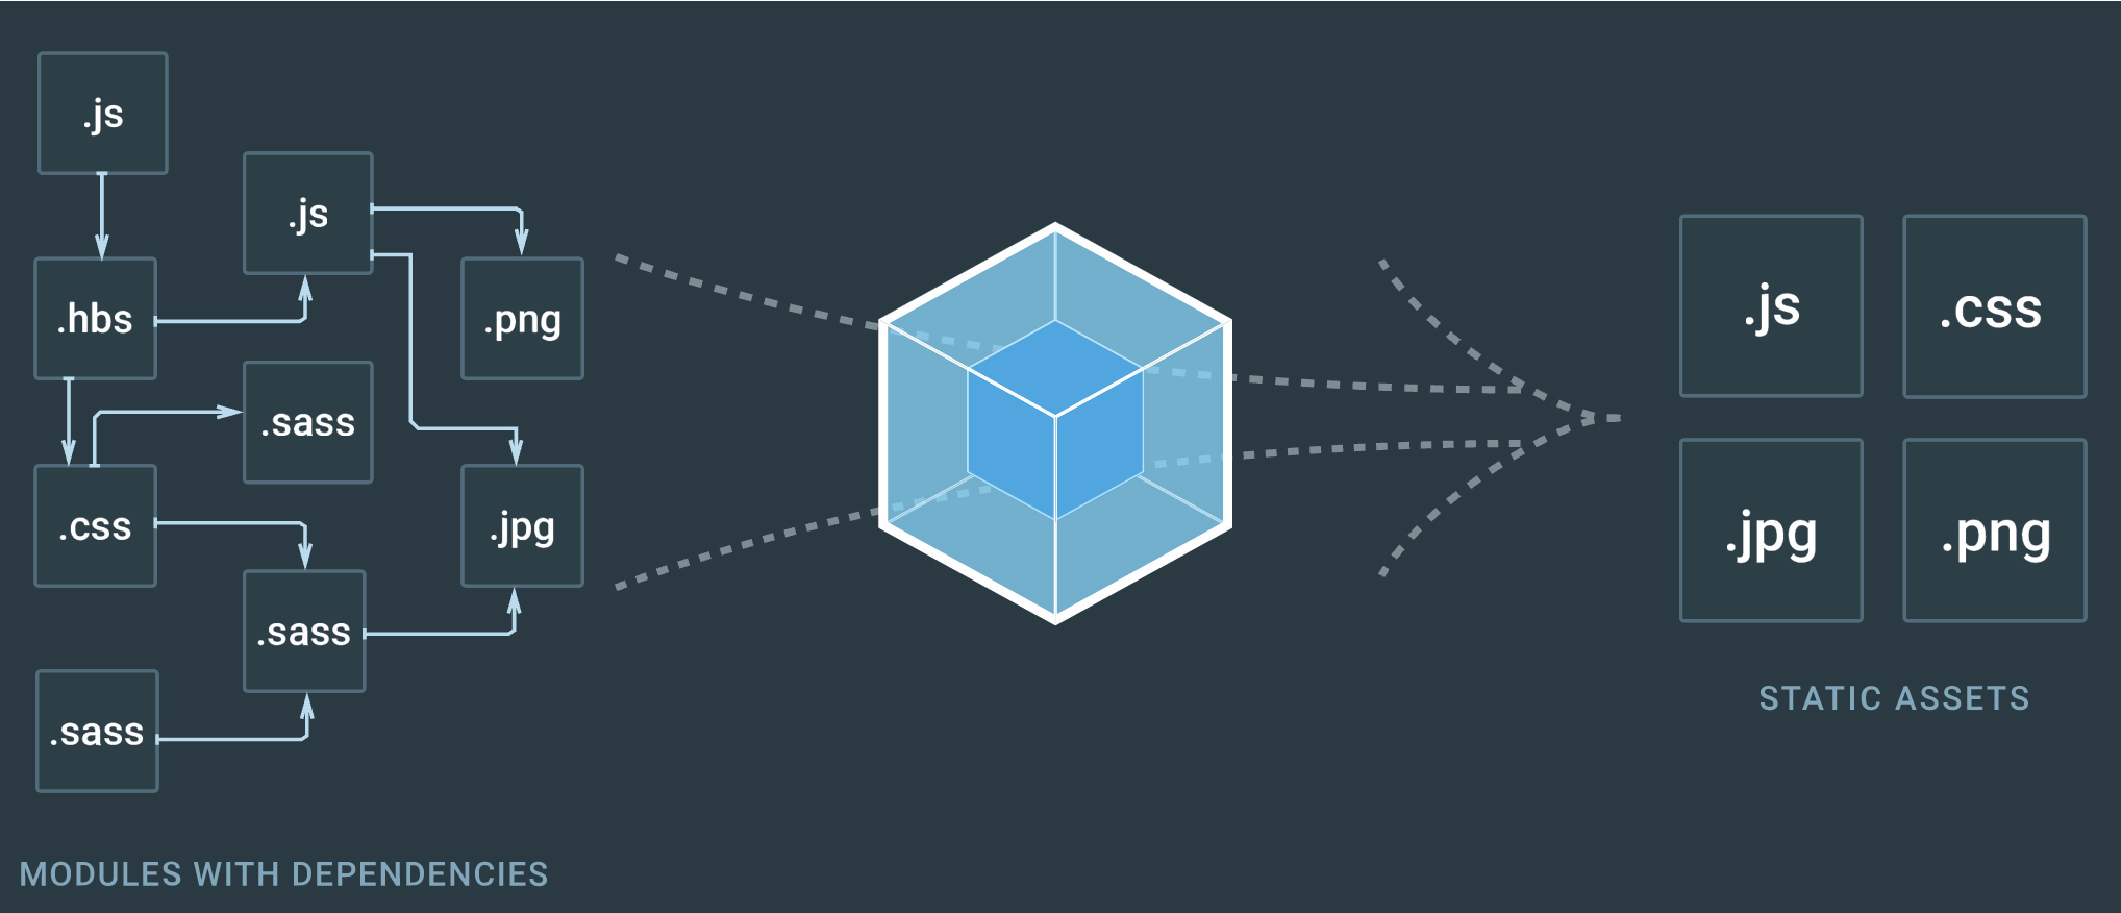
\includegraphics[width=0.9\textwidth]{webpack}
\caption{Bundling dependencies and static assets with Webpack \ref{r:1}}
\label{r:1}
\end{figure}

\subsubsection{Math.js}
Math.js is an extensive math library for JavaScript and Node.js. It features a flexible expression parser with support for symbolic computation, comes with a large set of built-in functions and constants, and offers an integrated solution to work with different data types like numbers, big numbers, complex numbers, fractions, units, and matrices.

\subsection{Test-driven development}
Test-driven development (TDD), is an evolutionary approach to development which combines test-first development where we write a test before we write just enough production code to fulfill that test and refactoring. One view is the goal of TDD is specification and not validation.  In other words, it’s one way to think through our requirements or design before we write our functional code (implying that TDD is both an important agile requirements and agile design technique). Another view is that TDD is a programming technique. The goal of TDD is to write clean code that works.

\subsection{Virtual calculator entity}

\begin{figure}[ht!]
\centering
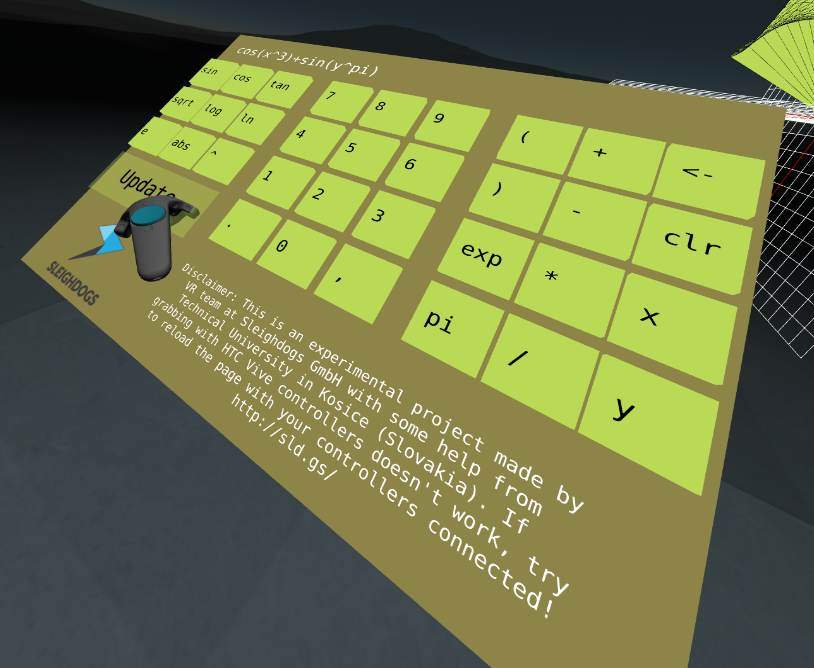
\includegraphics[width=0.6\textwidth]{calculator}
\caption{Virtual calculator entity \ref{r:2}}
\label{r:2}
\end{figure}

\subsubsection{Parsing equations with Math.js}

\subsection{Parametrized function grid entity}

\subsection{Interactive function settings panel entity}

\begin{figure}[ht!]
\centering
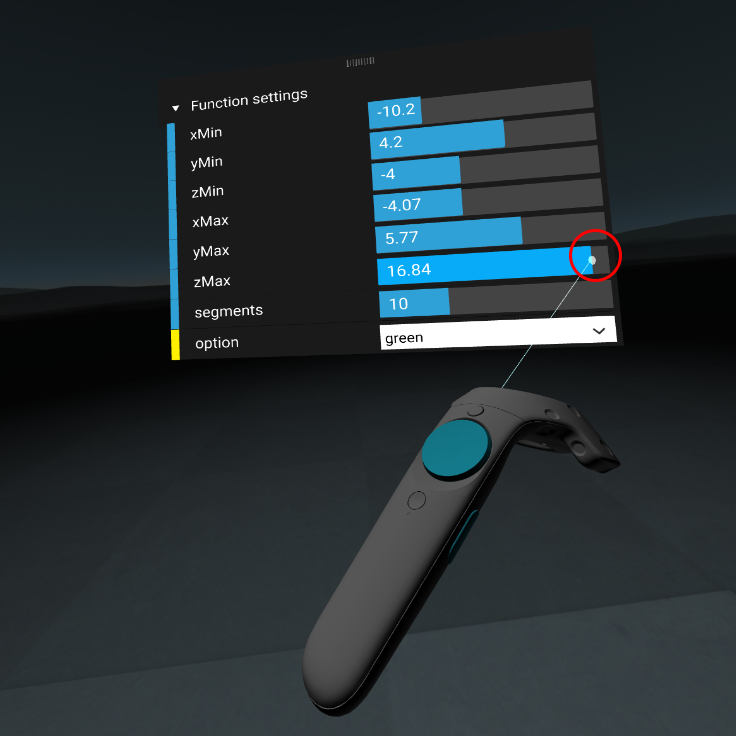
\includegraphics[width=0.6\textwidth]{function_settings}
\caption{Function settings entity \ref{r:4}}
\label{r:4}
\end{figure}

\subsection{Interactions}

\subsubsection{Grabbing}

\begin{figure}[ht!]
\centering
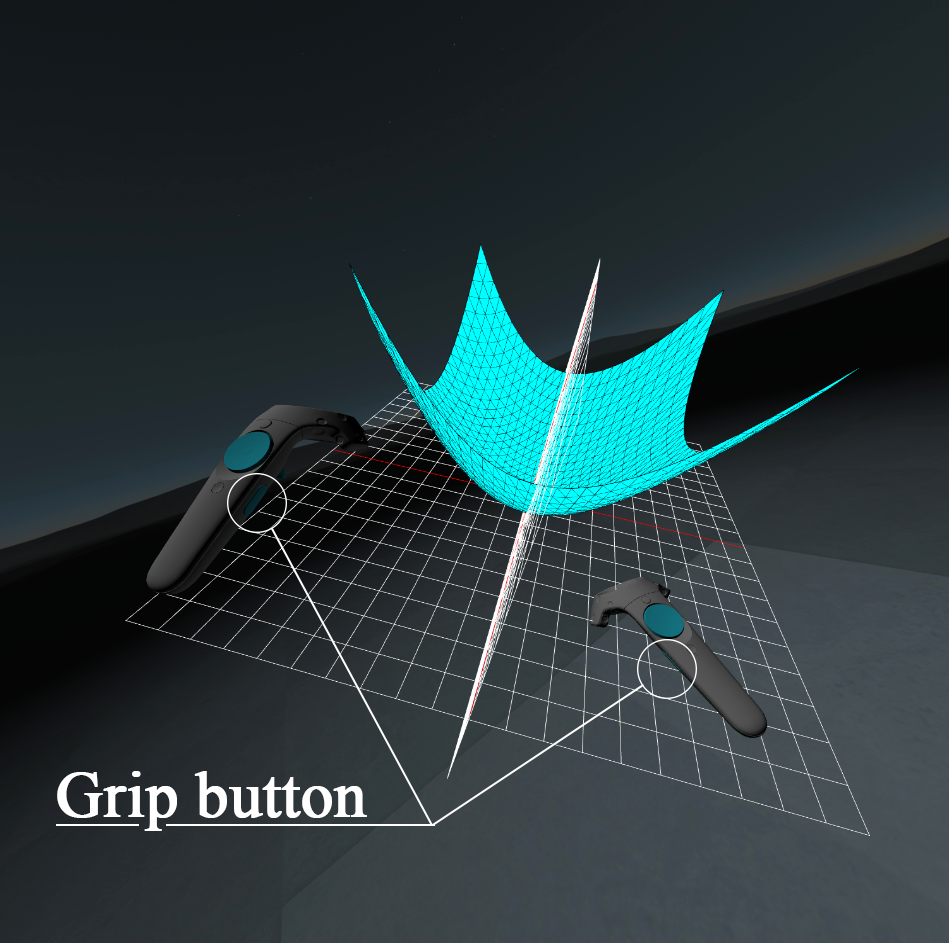
\includegraphics[width=0.6\textwidth]{grab}
\caption{Grabbing functionality \ref{r:5}}
\label{r:5}
\end{figure}

\subsubsection{Scaling}

\begin{figure}[ht!]
\centering
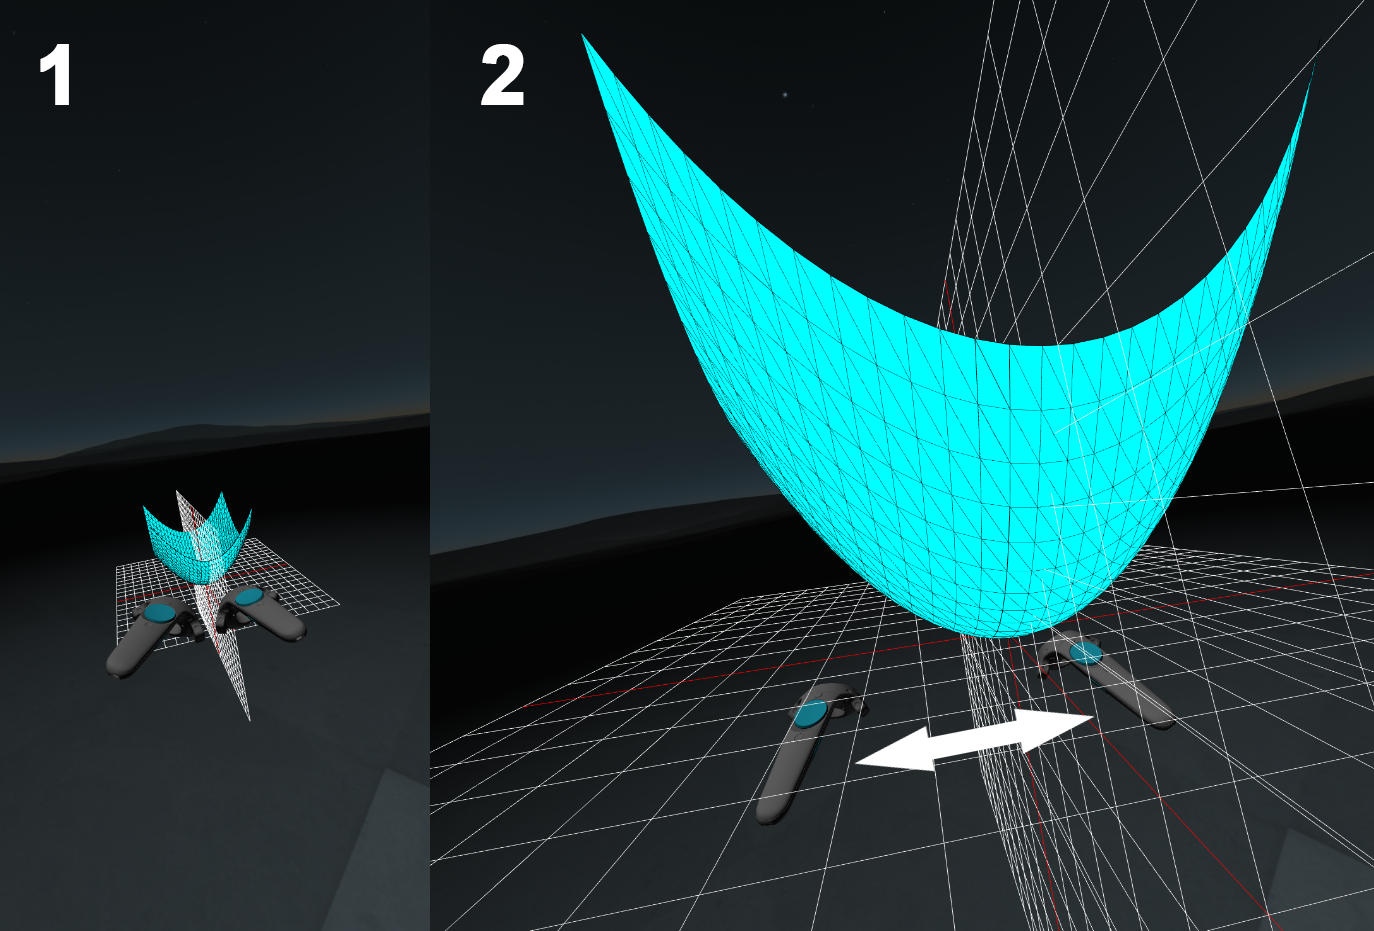
\includegraphics[width=0.6\textwidth]{scaling}
\caption{Scaling functionality \ref{r:6}}
\label{r:6}
\end{figure}

\subsection{Building and deploying the application to web hosting}


%Začnime rovnicou
%
%\begin{equation}\label{r:2}
%\frac{\ud^2y}{\ud t^2}+\frac{\ud y}{\ud t}+y =0, \qquad y(0)=1, \quad
%y\,'(0)=15.
%\end{equation}
%
%Grafický priebeh riešenia tejto rovnice vidíme na Obrázku \ref{o:2}.
%
%\begin{figure}[ht!]
%\centering
%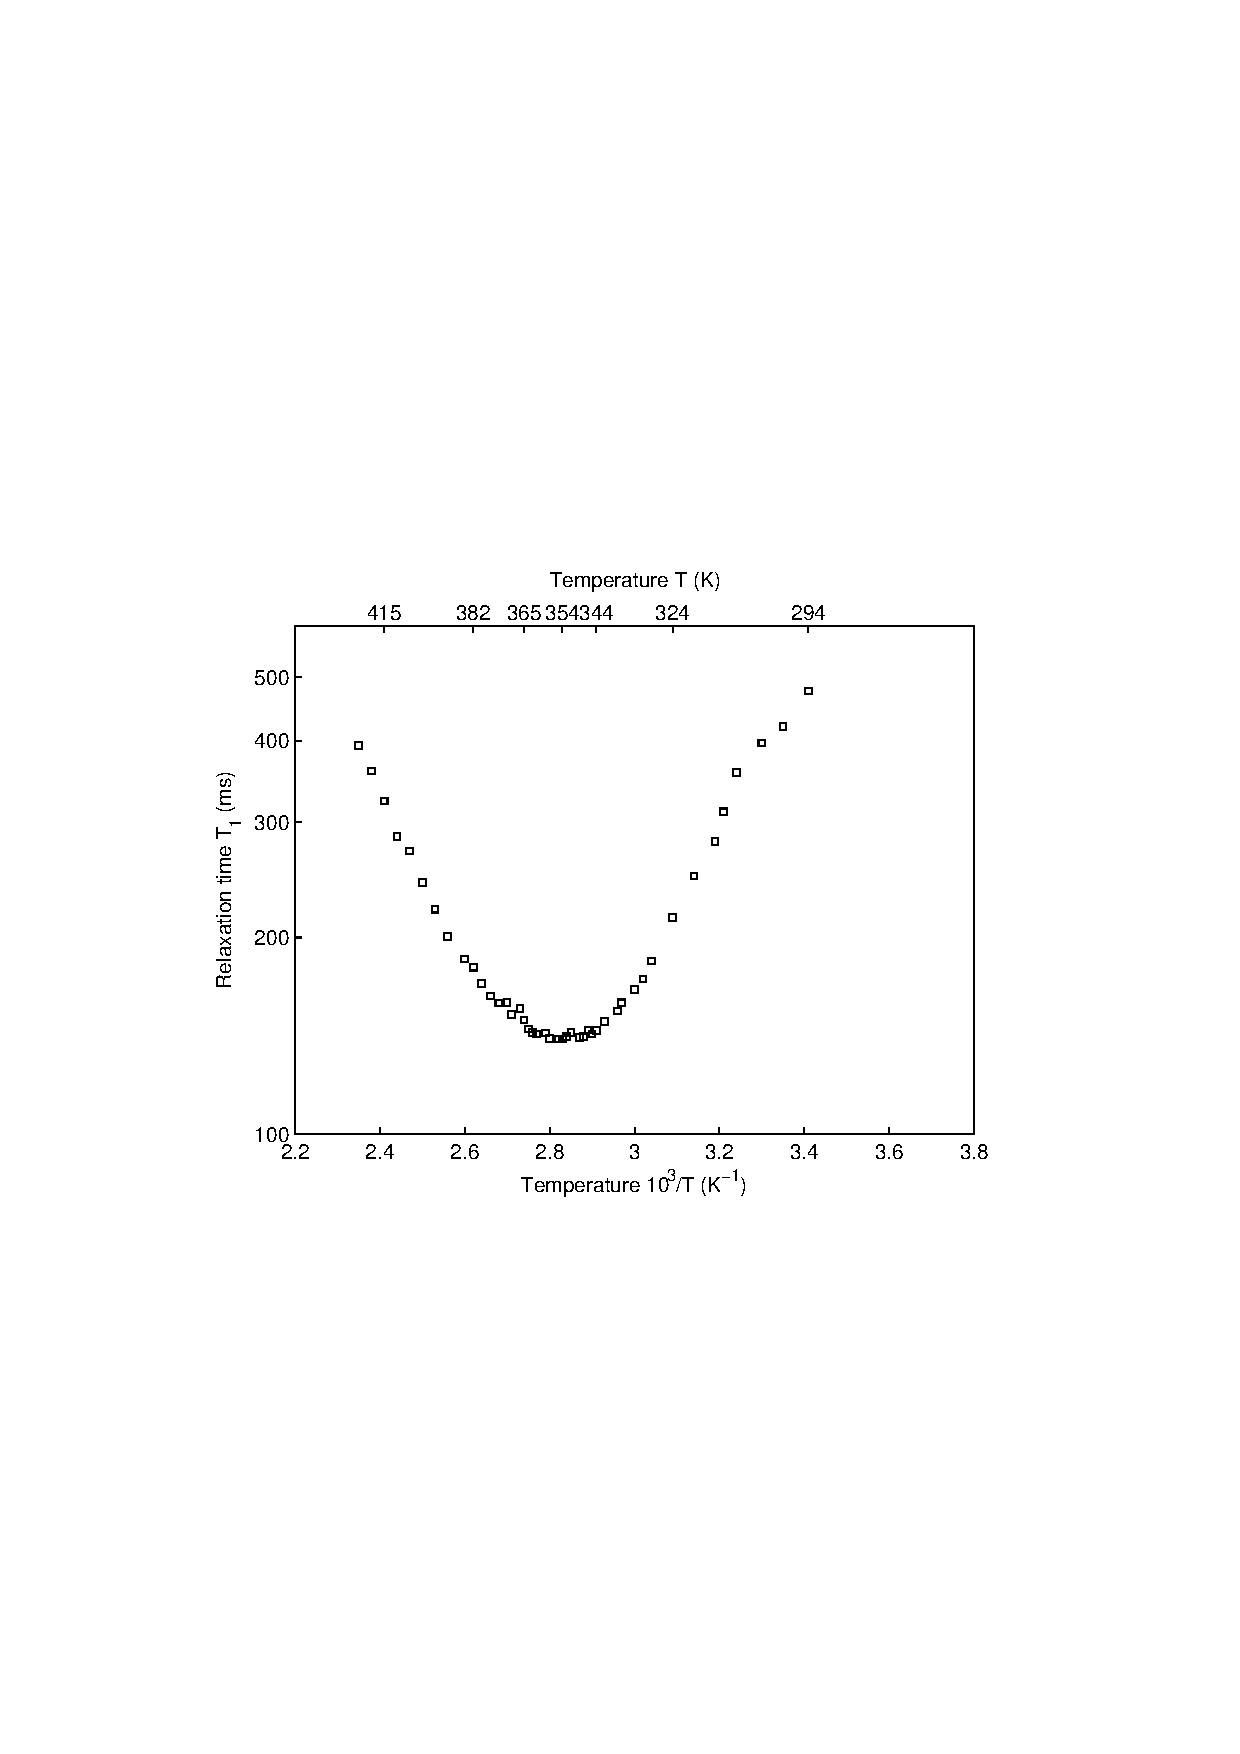
\includegraphics[width=.6\textwidth,angle=0]{relaxcas.pdf}
%\caption{Teplotná závislosť\/ spinovo-mriežkového relaxačného
%času}\label{o:3}
%\end{figure}
%
%%\tabcolsep=3pt % sirka stlpcov
%%\renewcommand{\arraystretch}{1.2} % riadkovanie
%\begin{table}[ht!]
%\centering
%\caption{Parametre získané z~meraní spinovo-mriežkových relaxačných
%časov $T_1$}\label{t:2}
%\medskip
%\newcolumntype{d}{D{,}{,}{-1}}
%\begin{tabular}{||c||d|d|d|d|d||}
%\hhline{|t:==t:==:==:t|}
%\multicolumn{1}{||c||}{}&\multicolumn{1}{c|}{PP --
%01}&\multicolumn{1}{c|}{PP -- 05}&\multicolumn{1}{c|}{PP --
%10}&\multicolumn{1}{c|}{PP -- 16}&\multicolumn{1}{c||}{PP -- 22} \\
%\hhline{|:==:==:==:|}
%C $\cdot 10^8$~(s$^{-2}$) & 10,1 & 10,0 & 11,0 & 9,2 & 8  \\
%\hhline{||-|-|-|-|-|-||}
%$\tau_0 \cdot 10^{-14}$~(s) & 2,63 & 1,44 & 0,95 & 2,21 & 10,83  \\
%\hhline{||-|-|-|-|-|-||}
%$E_{\text a}$~(kJ) & 34,26 & 8,33 & 39,76 & 37,31 & 31,86  \\
%\hhline{||-|-|-|-|-|-||}
%$T_{\min}$~(K) & 354 & 367 & 367 & 369 & 367  \\
%\hhline{||-|-|-|-|-|-||}
%$T_{1\min}$~(ms) & 141 & 160 & 157 & 175 & 181  \\
%\hhline{||-|-|-|-|-|-||}
%$\Delta M_2$~(Gs$^2$) & 5,49 & 5,66 & 5,16 & 5,09 & 5,02  \\
%\hhline{|b:==b:==:==:b|}
%\end{tabular}
%\end{table}

